\documentclass[paper=a4, fontsize=11pt]{scrartcl}

\usepackage[T1]{fontenc}
\usepackage[english]{babel}
\usepackage{amsmath,amsfonts,amsthm}
\usepackage{graphicx}
\usepackage{booktabs}
\usepackage{listings}
\usepackage{color}
\usepackage{lipsum}
\usepackage{sectsty}
\allsectionsfont{\centering \normalfont\scshape}
\usepackage{fancyhdr}
\pagestyle{fancyplain}
\fancyhead{}
\fancyfoot[L]{}
\fancyfoot[C]{}
\fancyfoot[R]{\thepage}
\renewcommand{\headrulewidth}{0pt}
\renewcommand{\footrulewidth}{0pt}
\setlength{\headheight}{13.6pt}

\numberwithin{equation}{section}
\numberwithin{figure}{section}
\numberwithin{table}{section}

\setlength\parindent{0pt}

\definecolor{mygreen}{rgb}{0,0.6,0}
\definecolor{mygray}{rgb}{0.5,0.5,0.5}
\definecolor{mymauve}{rgb}{0.58,0,0.82}

\lstset{ %
  backgroundcolor=\color{white},   % choose the background color
  basicstyle=\footnotesize,        % size of fonts used for the code
  breaklines=true,                 % automatic line breaking only at whitespace
  captionpos=b,                    % sets the caption-position to bottom
  commentstyle=\color{mygreen},    % comment style
  escapeinside={\%*}{*)},          % if you want to add LaTeX within your code
  keywordstyle=\color{blue},       % keyword style
  stringstyle=\color{mymauve},     % string literal style
}

%----------------------------------------------------------------------------------------
%	TITLE SECTION
%----------------------------------------------------------------------------------------

\newcommand{\horrule}[1]{\rule{\linewidth}{#1}} % Create horizontal rule command with 1 argument of height

\title{	
\normalfont \normalsize 
\textsc{Escuela multimedial Da Vinci} \\ [25pt]
\textsc{Departamento de sistemas} \\ [25pt]
\horrule{0.5pt} \\[0.4cm]
\huge Unidad 3 - Guia de ejercicios\\
\horrule{2pt} \\[0.5cm]
}

\author{David Alejandro Trejo Pizzo}
\date{\normalsize\today}

\begin{document}

\maketitle

%----------------------------------------------------------------------------------------
%	PROBLEMA 1
%----------------------------------------------------------------------------------------

\section{Ciclo While}

\lipsum[2] % Dummy text

Sometimes you want everything in the program to stop while a given condition is true. You can do this using a while loop. This example shows how to use a while loop to calibrate the value of an analog sensor.
In the main loop, the sketch below reads the value of a photoresistor on analog pin 0 and uses it to fade an LED on pin 9. But while a button attached to digital pin 2 is pressed, the program runs a method called calibrate() that looks for the highest and lowest values of the analog sensor. When you release the button, the sketch continues with the main loop.
This technique lets you update the maximum and minimum values for the photoresistor when the lighting conditions change.

\subsection{Hardware Required}

Arduino Board
(1) digital pushbutton or switch
(1) photocell, or analog sensor
(2) 10k ohm resistors
breadboard

\subsection{Circuito}

Connect your analog sensor (e.g. potentiometer, light sensor) on analog input 2 with a 10K ohm resistor to ground. Connect your button to digital pin, again with a 10K ohm resistor to ground. Connect your LED to digital pin 9, with a 220 ohm resistor in series.

\begin{figure}[!h]
\centering
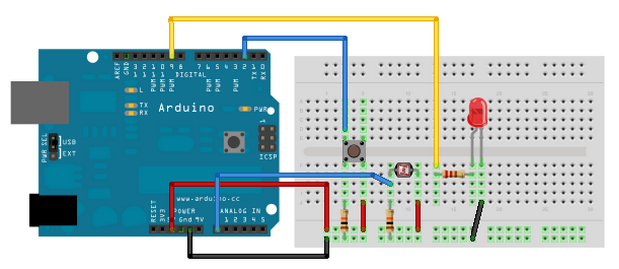
\includegraphics[width=4in]{circuito1}
\end{figure}

\subsection{Code}

\begin{lstlisting}[language=java]

// These constants won't change:
const int sensorPin = A2;       // pin that the sensor is attached to
const int ledPin = 9;           // pin that the LED is attached to
const int indicatorLedPin = 13; // pin that the built-in LED is attached to
const int buttonPin = 2;        // pin that the button is attached to


// These variables will change:
int sensorMin = 1023;  // minimum sensor value
int sensorMax = 0;     // maximum sensor value
int sensorValue = 0;         // the sensor value


void setup() {
  // set the LED pins as outputs and the switch pin as input:
  pinMode(indicatorLedPin, OUTPUT);
  pinMode (ledPin, OUTPUT);
  pinMode (buttonPin, INPUT);
}

void loop() {
  // while the button is pressed, take calibration readings:
  while (digitalRead(buttonPin) == HIGH) {
    calibrate(); 
  }
  // signal the end of the calibration period
  digitalWrite(indicatorLedPin, LOW);  

  // read the sensor:
  sensorValue = analogRead(sensorPin);

  // apply the calibration to the sensor reading
  sensorValue = map(sensorValue, sensorMin, sensorMax, 0, 255);

  // in case the sensor value is outside the range seen during calibration
  sensorValue = constrain(sensorValue, 0, 255);

  // fade the LED using the calibrated value:
  analogWrite(ledPin, sensorValue);
}

void calibrate() {
  // turn on the indicator LED to indicate that calibration is happening:
  digitalWrite(indicatorLedPin, HIGH);
  // read the sensor:
  sensorValue = analogRead(sensorPin);

  // record the maximum sensor value
  if (sensorValue > sensorMax) {
    sensorMax = sensorValue;
  }

  // record the minimum sensor value
  if (sensorValue < sensorMin) {
    sensorMin = sensorValue;
  }
}
\end{lstlisting}

%----------------------------------------------------------------------------------------
%	PROBLEM 2
%----------------------------------------------------------------------------------------

\section{Lists}

%------------------------------------------------

\subsection{Example of list (3*itemize)}
\begin{itemize}
	\item First item in a list 
		\begin{itemize}
		\item First item in a list 
			\begin{itemize}
			\item First item in a list 
			\item Second item in a list 
			\end{itemize}
		\item Second item in a list 
		\end{itemize}
	\item Second item in a list 
\end{itemize}

%------------------------------------------------

\subsection{Example of list (enumerate)}
\begin{enumerate}
\item First item in a list 
\item Second item in a list 
\item Third item in a list
\end{enumerate}

%----------------------------------------------------------------------------------------

\end{document}